\chapter{Mathematical Modeling and Theoretical Framework}
\label{ch:chapter3}


\section{3.1  Introduction}
This chapter establishes the mathematical foundations for the proposed DWT-LSTM transformer differential protection scheme, covering differential relaying principles (Section 3.2), magnetizing inrush theory (Section 3.3), CT saturation modeling (Section 3.4), internal fault characteristics (Section 3.5), and the classification framework (Section 3.6).


\section{3.2  Transformer Differential Protection Fundamentals}

\subsection{3.2.1  Differential Current and Restraint Current}
For a two-winding transformer, the differential and restraint currents are defined as:

I\_d = | İ1·N1 + İ2·N2 |	(3.1)

I\_r = ( |İ1·N1| + |İ2·N2| ) / 2	(3.2)

where İ1, İ2 are phasor currents referred to the same voltage level and N1, N2 are CT ratios. Under healthy conditions I\_d ≈ 0; a small residual arises from CT mismatch, tap-changer effects, magnetizing current, and measurement errors:

I\_d,steady = √[ (ε\_CT·I\_load)² + (Δ\_tap·I\_load)² + I\_m² + ε\_meas² ]	(3.3)


\subsection{3.2.2  Operating Characteristics}
The dual-slope restraint characteristic defines the operating threshold I\_op as a function of restraint current I\_r, with pickup I\_pickup, first slope S1 (25--40\%) accommodating steady-state errors, and second slope S2 (50--80\%) providing additional restraint during CT saturation from through-faults. The relay trips when:

I\_d > I\_op	(3.4)

Figure 3.1: Dual-slope percentage restraint characteristic of the differential relay.


\subsection{3.2.3  Pickup Current}
The pickup must balance sensitivity and security, I\_d,steady,max < I\_pickup < I\_d,fault,min, typically set to 0.2--0.5 p.u. The minimum detectable SLG fault current referred to the primary is I\_f,min = I\_pickup / [1 - R\_f/(Z\_s,pu + Z\_t,pu)].


\section{3.3  Magnetizing Inrush Current Phenomenon}

\subsection{3.3.1  Core Saturation Theory}
Inrush results from transient core saturation upon transformer energization. Faraday's law gives v(t) = N dφ/dt = NA dB/dt. For sinusoidal voltage v(t) = V\_m sin(ωt + α), the steady-state flux is φ\_ss(t) = -Φ\_m cos(ωt + α). Including the DC transient:

φ(t) = -Φ\_m cos(ωt + α) + Φ\_m cos(α) e^(-t/τ) + Φ\_r e^(-t/τ)	(3.5)

At worst-case energization (α = 0, Φ\_r = Φ\_m), the peak flux Φ\_peak = 2Φ\_m + Φ\_r = 3Φ\_m, exceeding B\_sat and causing severe saturation.

Figure 3.2: Core B-H saturation curve and the resulting magnetizing inrush waveform.


\subsection{3.3.2  Factors Affecting Inrush}
Inrush magnitude depends on switching angle α, residual flux Φ\_r (0--80\% of Φ\_m), source impedance Z\_s, core material, and transformer rating. Typical inrush ranges from 3--15× rated current, with peak flux Φ\_peak(α) = Φ\_m(1 + |cos α|) + Φ\_r cos α.


\subsection{3.3.3  Harmonic Characteristics}
The asymmetric inrush waveform contains both odd and even harmonics. The second harmonic dominates the even spectrum (15--60\% for silicon steel; 7--12\% for amorphous alloys). The key harmonic restraint ratios are k2 = (I2/I1)×100\% and k5 = (I5/I1)×100\%.


\subsection{3.3.4  Sympathetic Inrush}
Sympathetic inrush occurs when an energizing transformer's DC inrush current, flowing through the common source impedance, drives an already-energized parallel transformer into opposite-polarity saturation, producing a slowly decaying differential current. The coupled DC circuit equations yield two exponential decay modes with combined time constants, producing sympathetic inrush that can persist for tens of seconds \cite{ref4}.


\section{3.4  Current Transformer Saturation Model}

\subsection{3.4.1  CT Equivalent Circuit}
The CT secondary current equals the referred primary minus the excitation current through the nonlinear magnetizing branch, I\_s = I\_p′ - I\_e, with I\_e = V\_s/(R\_m + jX\_m) and V\_s = I\_s(R\_s + jX\_s + Z\_b). The nonlinear magnetization curve uses the exponential model i\_e(λ) = A e^(B|λ|) sign(λ) + Cλ, where flux linkage λ = N2·φ = L\_m(I\_e)·I\_e and v\_s = dλ/dt.

Figure 3.3: Current transformer equivalent circuit and saturation-induced secondary distortion.


\subsection{3.4.2  Transient DC Offset and Flux Buildup}
CT saturation is caused by DC offset in fault currents, i\_p(t) = I\_m[sin(ωt + α - φ) - sin(α - φ) e^(-t/τ\_f)]. The core flux comprises AC and DC components; saturation occurs when λ > λ\_sat. The time to saturation t\_sat decreases with higher fault current, maximum DC offset, larger remanent flux, and higher burden.


\subsection{3.4.3  Impact on Differential Protection}
Asymmetric CT saturation during external faults produces spurious differential current I\_d = |I\_e1 - I\_e2| ≠ 0. When one CT remains unsaturated, the maximum spurious current is approximately I\_d,max ≈ I\_fault · (R\_b2 + R\_s2)/(R\_b2 + R\_s2 + Z\_m2). The second slope S2 of the restraint characteristic provides the necessary restraint.


\section{3.5  Internal Fault Characteristics}

\subsection{3.5.1  Types of Internal Faults}
Internal faults include phase-to-ground (SLG, most common), phase-to-phase (LL), three-phase (LLL/LLLG), and inter-turn faults. Inter-turn faults are hardest to detect since shorted turns partially cancel the affected MMF, I\_d ≈ (N\_s/N)·I\_load; for 1--5\% turn faults, I\_d may fall below load-current level.


\subsection{3.5.2  Fault Current Analysis}
Using symmetrical components, an SLG fault on phase a with impedance Z\_f yields I\_a1 = I\_a2 = I\_a0 = V\_f/(Z1 + Z2 + Z0 + 3Z\_f). For a phase-to-phase fault between phases b and c, I\_a1 = -I\_a2 = V\_f/(Z1 + Z2). The transient fault current contains a decaying DC component, i\_f(t) = √2·I\_rms[sin(ωt + α - φ) - sin(α - φ) e^(-t/τ\_f)]. Fault time constants (0.02--0.05 s) are shorter than inrush (0.1--0.5 s), and fault currents have significantly lower even-harmonic content.


\section{3.6  Mathematical Framework for Classification}

\subsection{3.6.1  Feature Space Formulation}
Event classification is formulated as a pattern-recognition problem. The DWT-LSTM feature vector at time step t comprises the mean, standard deviation, and energy of DWT coefficients at each level. The wavelet energy at level k is:

E\_{Dk} = Σ\_n |D\_k[n]|²	(3.6)

The optimal classifier maximizes the posterior probability (Bayes' rule), ĉ = argmax\_c P(ω\_c|x) = argmax\_c p(x|ω\_c) P(ω\_c)/p(x). The LSTM learns this mapping through a softmax output and cross-entropy loss:

P(ω\_c | x\_{1:T}) = e^{z\_c} / Σ\_k e^{z\_k}	(3.7)

L = -(1/N) Σ\_n Σ\_c y\_{n,c} ln P(ω\_c | x\_{1:T})	(3.8)

Feature separability is guided by the Fisher discriminant ratio, FDR = (μ\_c1 - μ\_c2)² / (σ\_c1² + σ\_c2²).


\subsection{3.6.2  Performance Metrics}
Classification performance is evaluated using confusion-matrix-derived metrics: Accuracy = Σ\_c TP\_c / N\_total; Precision\_c = TP\_c/(TP\_c + FP\_c); Recall\_c = TP\_c/(TP\_c + FN\_c); and the F1-score F1\_c = 2·Precision\_c·Recall\_c/(Precision\_c + Recall\_c). For protection applications, Dependability = TP\_fault/(TP\_fault + FN\_fault) and Security = TN\_fault/(FP\_fault + TN\_fault) are paramount. Additional metrics include the Matthews Correlation Coefficient, operating time T\_op = t\_trip - t\_event (within 20--40 ms at 50 Hz), and the AUC-ROC.


\section{3.7  Adaptive Threshold and Decision-Theoretic Foundations}

\subsection{3.7.1  Bayes-Optimal Decision Boundary}
The four-class discrimination problem can be cast in a decision-theoretic framework that makes explicit the cost asymmetry inherent to protection. Let the class-conditional densities of the feature vector x be p(x | ω\_c) for c ∈ {internal, external, inrush, normal}, with priors P(ω\_c). The Bayes risk associated with deciding class i when the true class is j is encoded by a loss matrix L\_{ij}. The optimal decision minimises the conditional risk:

R(α\_i | x) = Σ\_j L\_{ij} P(ω\_j | x)	(3.10)

For protection, the loss of failing to detect an internal fault (a missed trip, FN) vastly exceeds the loss of a spurious trip (FP), which in turn exceeds the loss of an inter-class confusion among non-internal events. Encoding L\_{FN} ≫ L\_{FP} ≫ L\_{other} biases the boundary toward dependability, mathematically formalising the engineering imperative that no internal fault may go undetected. The hybrid architecture of Chapter 5 realises this asymmetry structurally: the LSTM is permitted to veto (raise security) only after the classical 87T element has asserted a fault, so the dependability floor is set by the certified relay rather than by the learned model.


\subsection{3.7.2  Adaptive Pickup as a Function of Operating State}
Conventional relays employ a fixed pickup I\_pickup. An adaptive formulation lets the threshold track the estimated steady-state error envelope so that sensitivity is maximised at light load and security is maximised during through-faults. A representative adaptive law is:

I\_pickup(t) = I\_p0 + k\_1 I\_r(t) + k\_2 σ̂\_d(t)	(3.11)

where I\_p0 is the base pickup, I\_r(t) the instantaneous restraint current, σ̂\_d(t) an online estimate of the differential-current noise standard deviation, and k\_1, k\_2 tuning coefficients. The term k\_1 I\_r(t) reproduces the classical percentage slope, while k\_2 σ̂\_d(t) inflates the threshold transiently when CT saturation or measurement noise elevates the differential-current variance. In the proposed scheme, this adaptive 87T element supplies the binary dependability signal, and the LSTM confidence score Conf(t) provides the complementary security signal, the two being combined in the handshake of Equation (5.1).


\subsection{3.7.3  Information-Theoretic Feature Separability}
Beyond the Fisher discriminant ratio of Section 3.6, the discriminative value of a feature can be quantified by the mutual information between the feature and the class label, I(X; Y) = H(Y) - H(Y | X), where H(·) denotes Shannon entropy. A feature with high I(X; Y) reduces class uncertainty substantially and is therefore retained. The wavelet detail energies are expected to exhibit the highest mutual information because fault inception injects broadband high-frequency content that the detail sub-bands localise efficiently, whereas inrush concentrates energy near the second harmonic and steady-state operation produces negligible detail energy. This expectation is confirmed empirically in Chapter 6 (Section 6.2.3), where the three detail-energy features account for 72.3\% of the total mutual information.

Figure 3.4: Conceptual feature-space separation of the four event classes with cost-asymmetric decision boundaries.


\subsection{3.7.4  Operating-Time Bound}
The maximum permissible operating time T\_max is dictated by transformer through-fault withstand and downstream coordination. For a 50 Hz system, sub-cycle clearing (T\_op < 20 ms) is the design target; the thermal stress imposed on the winding during an internal fault scales with the integral ∫ i²(t) dt over the fault duration, so every millisecond of reduced clearing time directly lowers insulation degradation and mechanical force on the windings. The latency budget derived in Chapter 5 (Section 5.6.3) and validated in Chapter 6 (Section 6.4.3) demonstrates that the complete DWT--LSTM--hybrid pipeline satisfies this bound with substantial margin.


\begin{figure}[htpb]
\centering
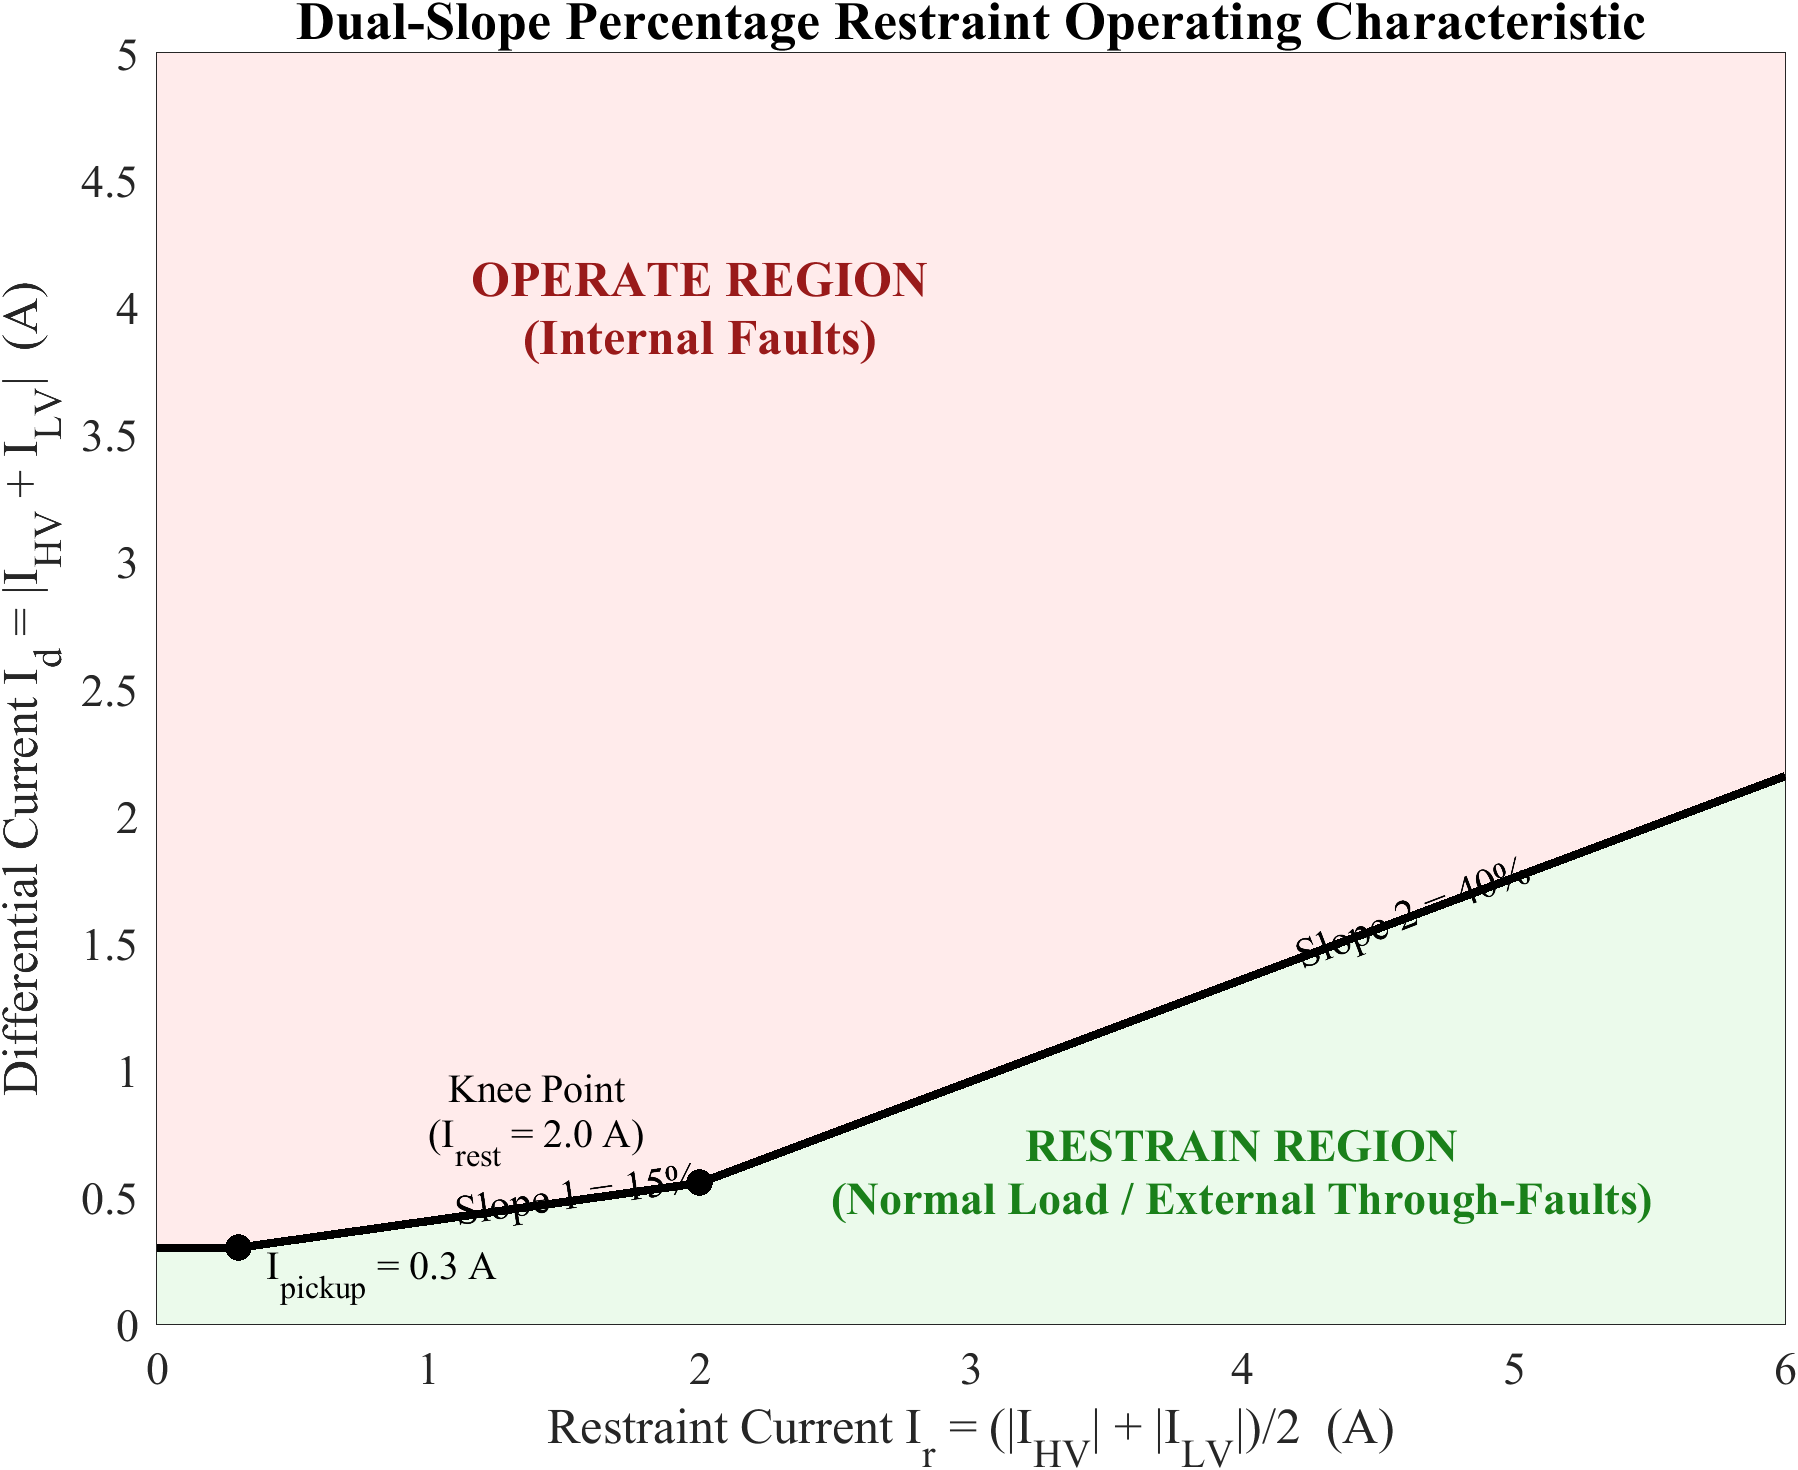
\includegraphics[width=0.75\textwidth]{figures/restraint_slope_characteristic.png}
\caption{Dual-slope percentage restraint characteristic of the differential relay.}
\label{fig:slope_char}
\end{figure}

\begin{figure}[htpb]
\centering
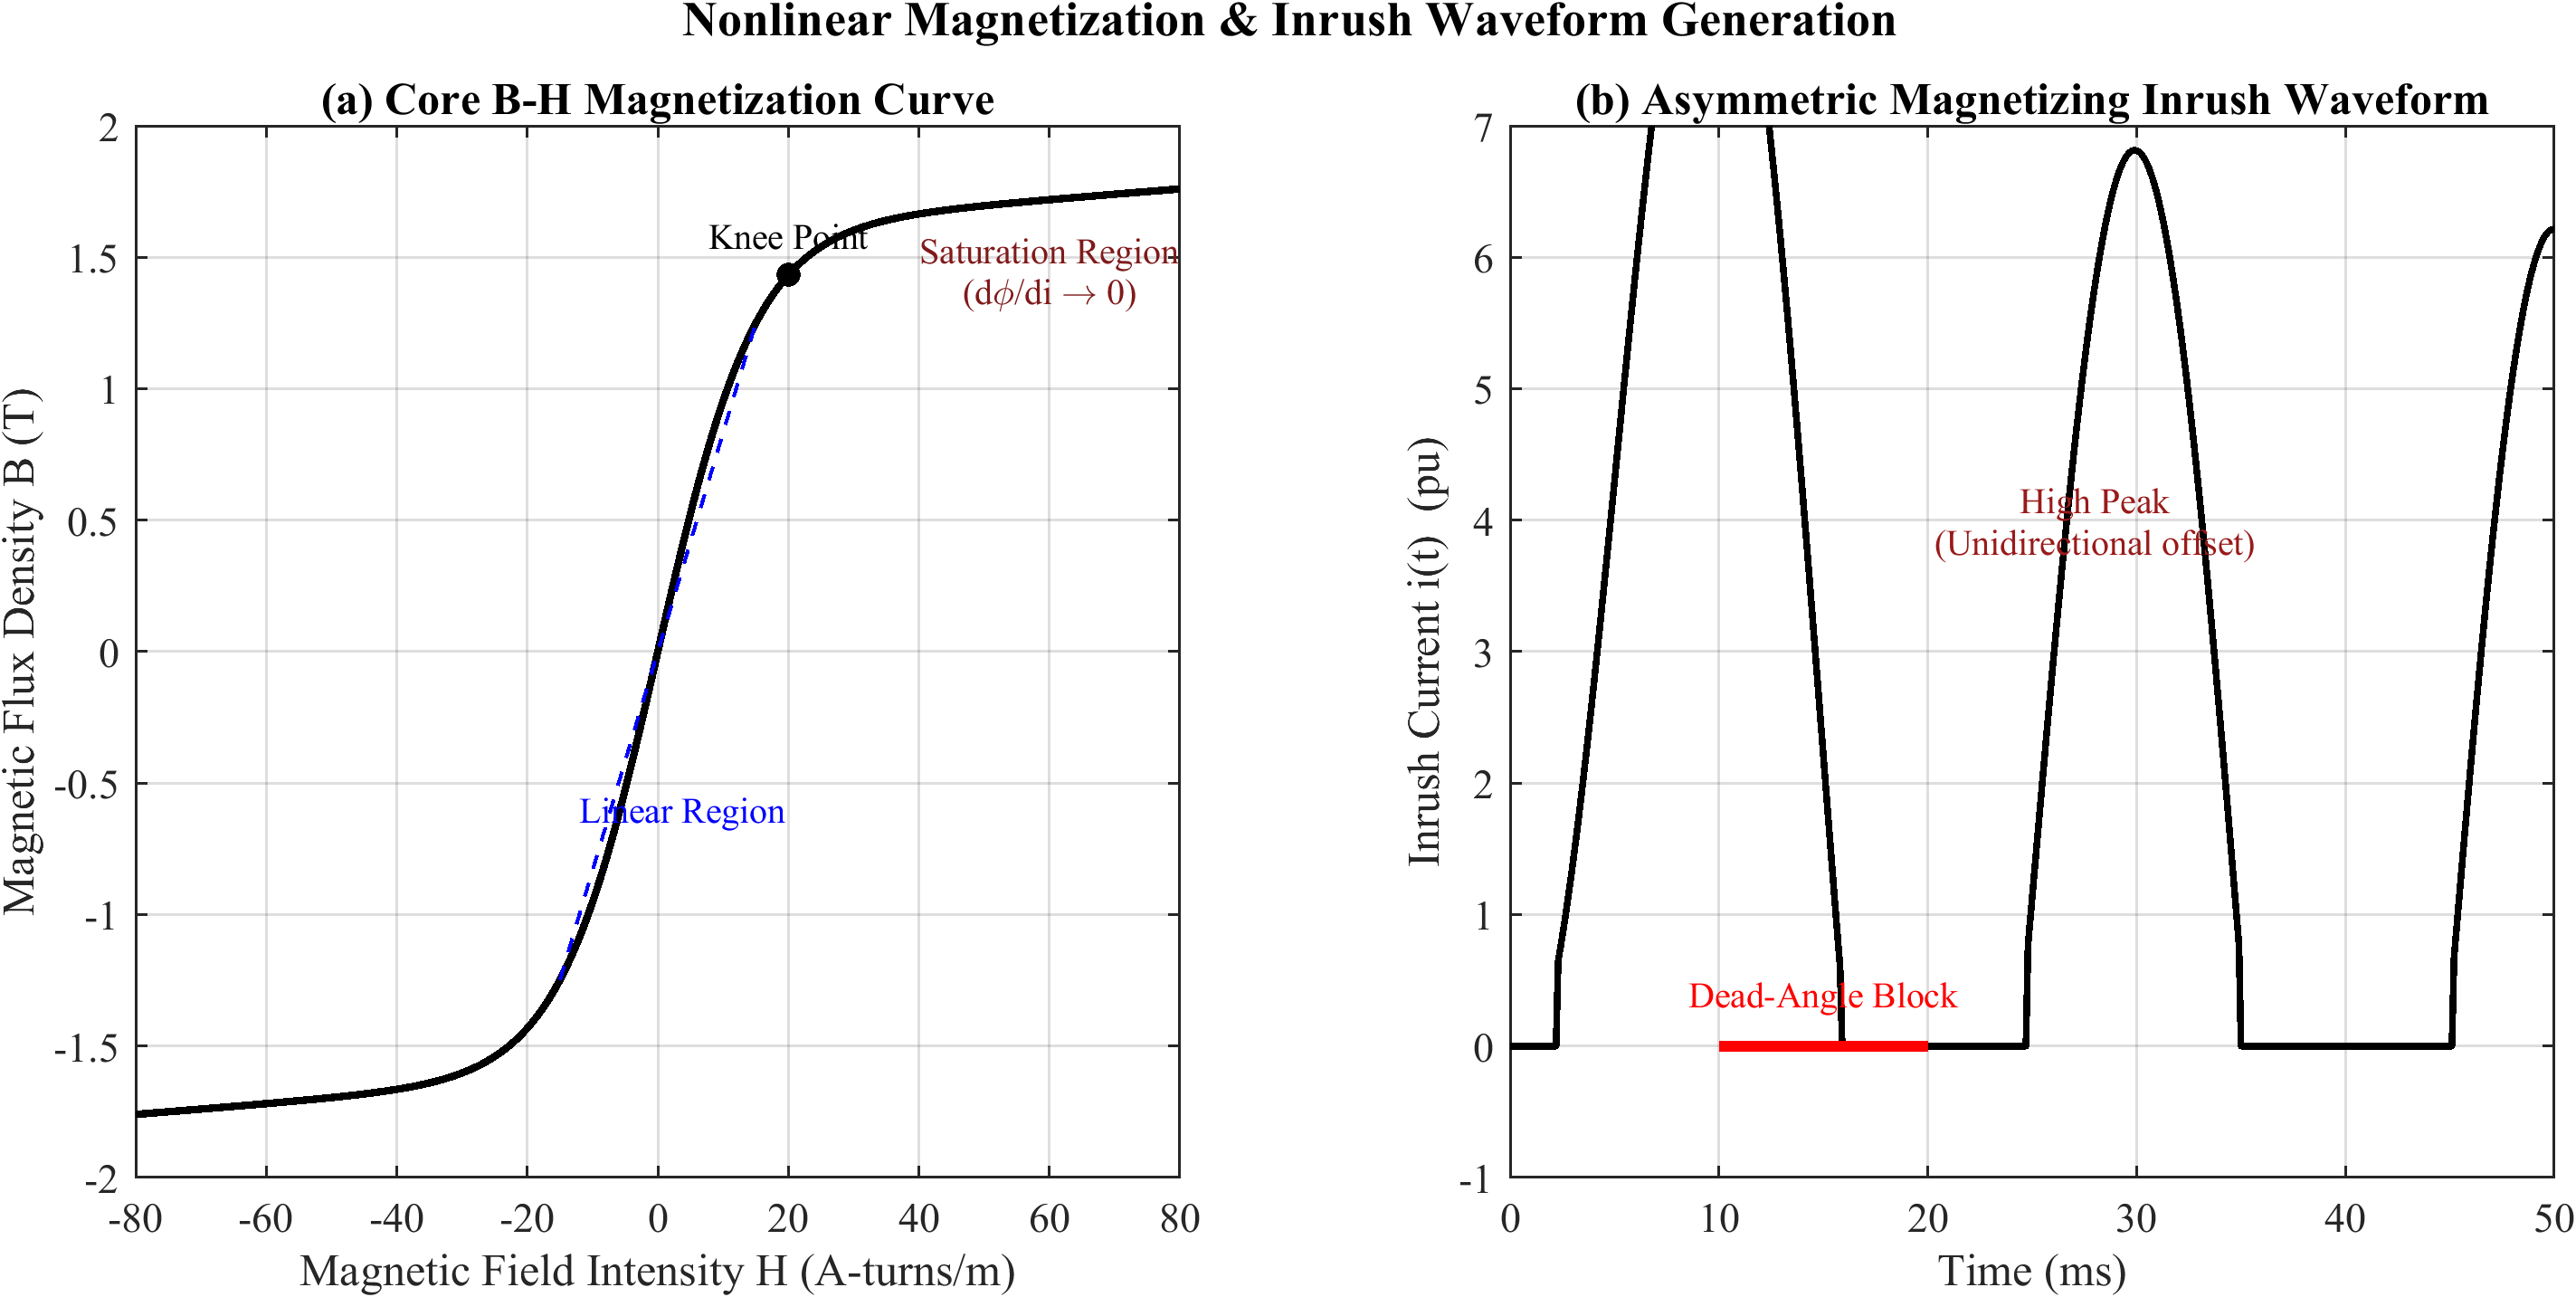
\includegraphics[width=0.75\textwidth]{figures/bh_and_inrush_characteristic.png}
\caption{Core B-H saturation curve and the resulting magnetizing inrush waveform.}
\label{fig:bh_inrush}
\end{figure}

\begin{figure}[htpb]
\centering
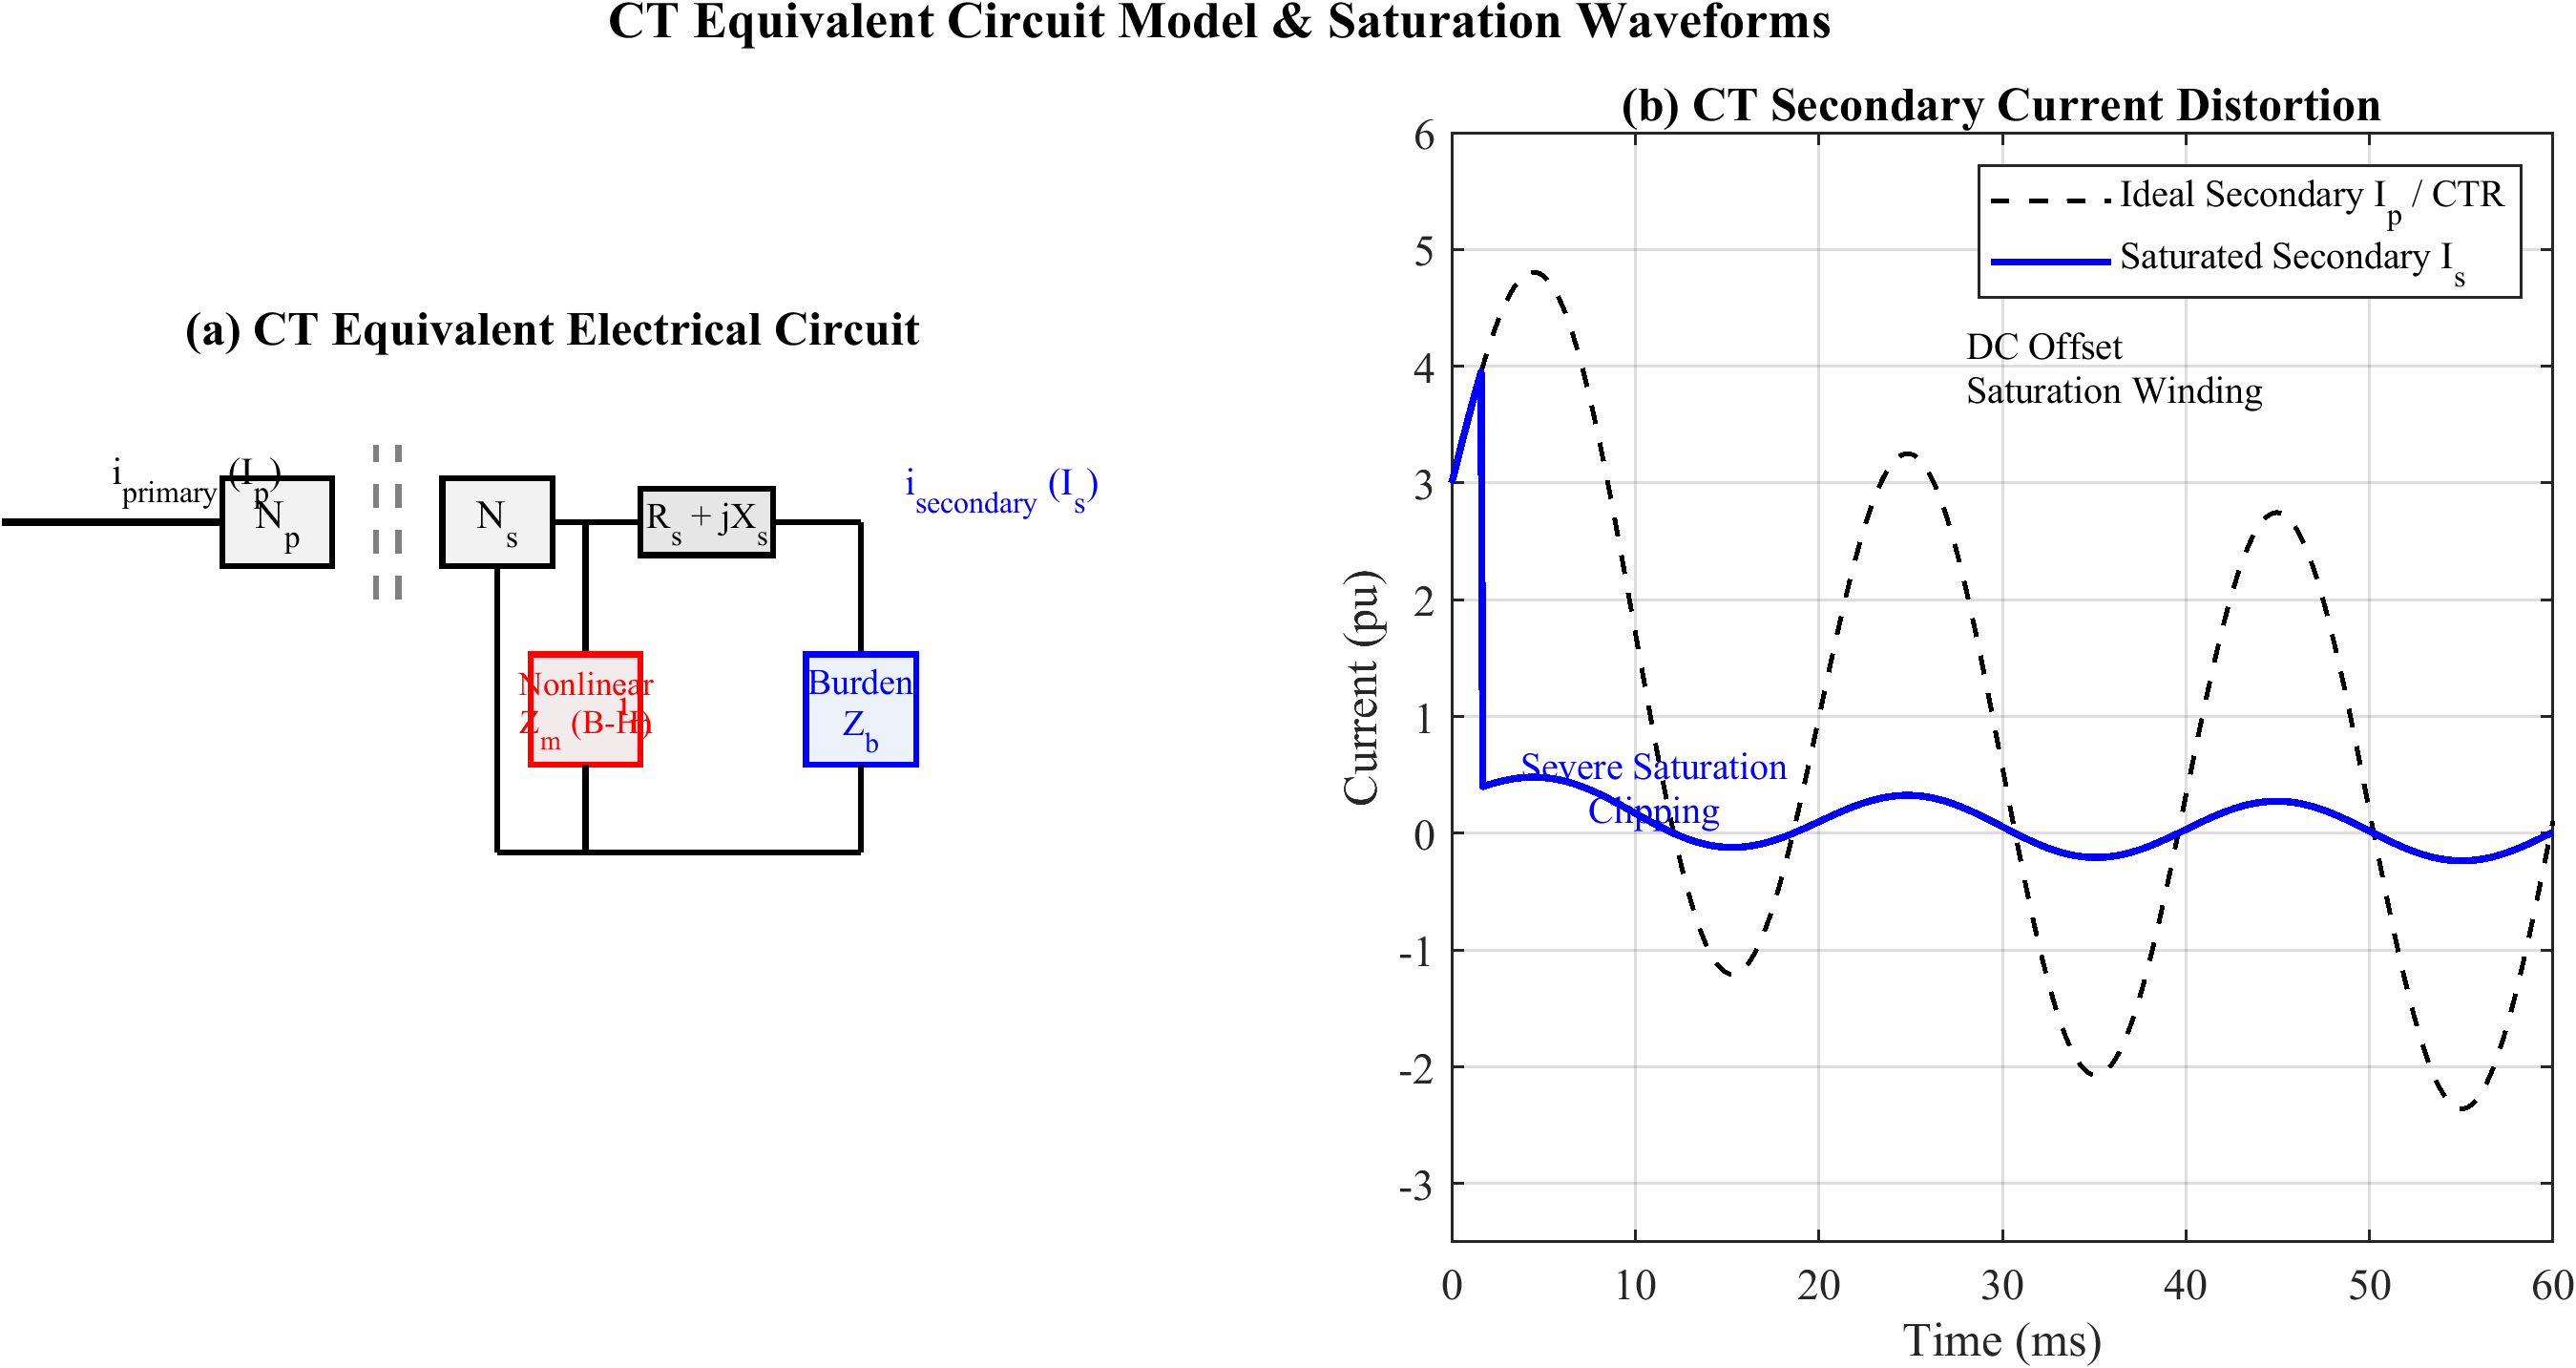
\includegraphics[width=0.75\textwidth]{figures/ct_saturation_characteristic.png}
\caption{Current transformer equivalent circuit and saturation-induced secondary distortion.}
\label{fig:ct_distortion}
\end{figure}

\begin{figure}[htpb]
\centering
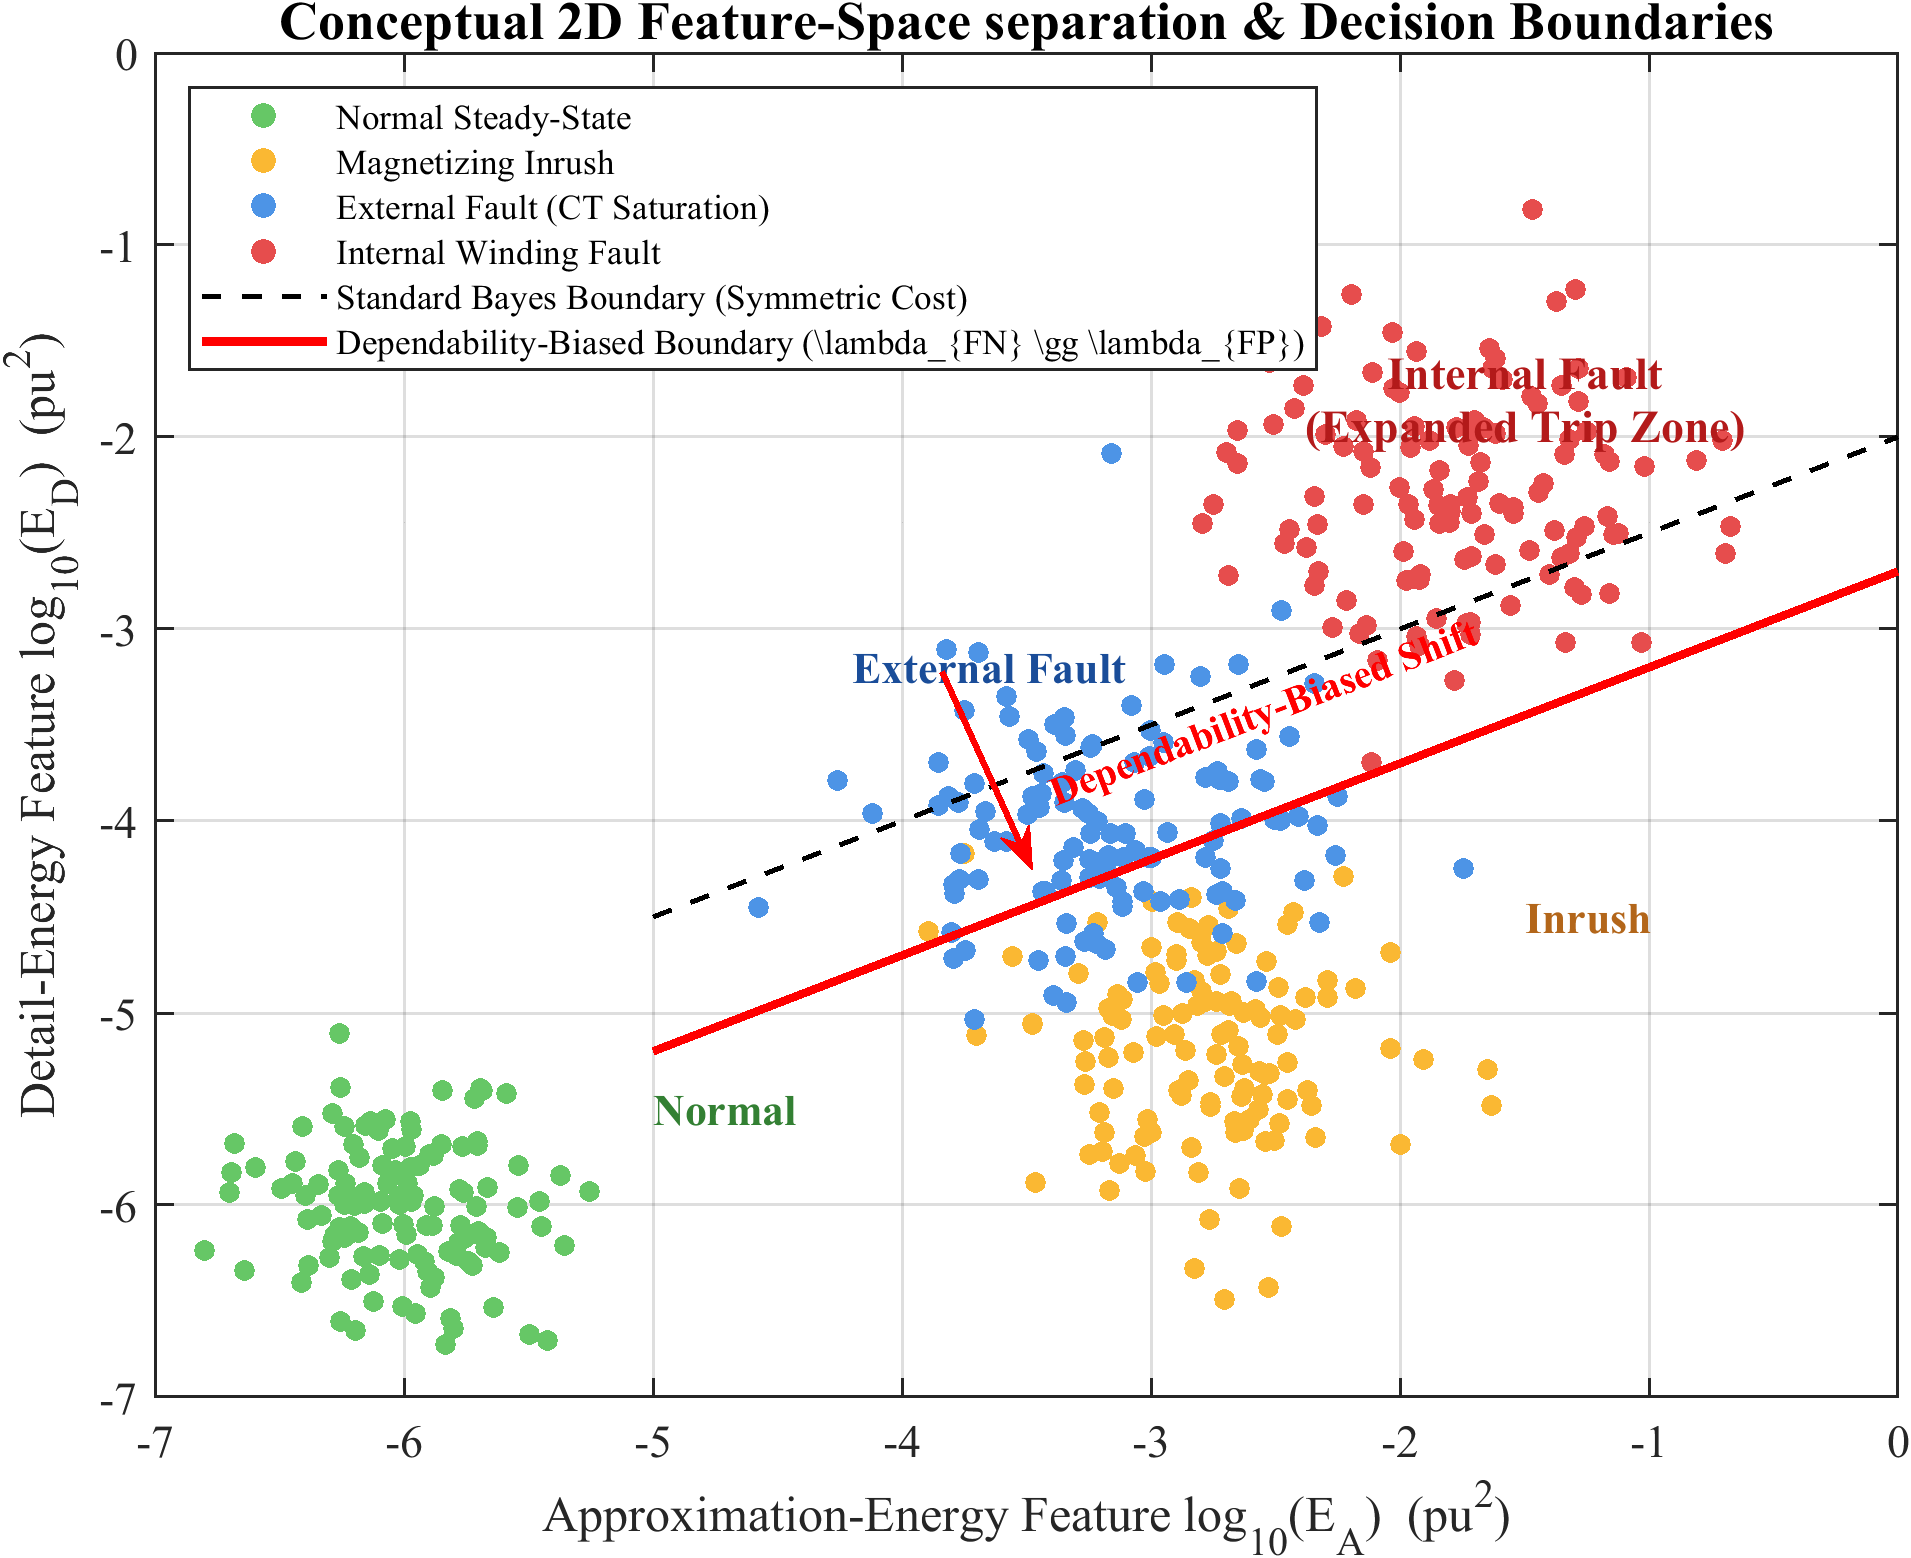
\includegraphics[width=0.75\textwidth]{figures/bayes_decision_boundary.png}
\caption{Conceptual feature-space separation of the four event classes with cost-asymmetric decision boundaries.}
\label{fig:bayes_boundary}
\end{figure}
